\documentclass{article}
\usepackage{../coursenotes}

\title{CSE 440 - Compiler Construction I}
\author{
{\Large Instructor: Dr. Rida Bazzi} \\
		Notes written by Brett Hansen
}
\date{}

\begin{document}

\maketitle
\tableofcontents
\break

\section{Week of August 14th, 2016}
\subsection{Compiler Components}

\begin{enumerate}
	\item Syntax
	\begin{enumerate}
		\item Lexical Analysis
		\item Parsing
	\end{enumerate}
	\item Semantics
	\begin{enumerate}
		\item Type Checking \textit{(Project 1)}
		\item Code Generation
		\begin{enumerate}
			\item Intermediate Representation \textit{(Project 2)}
			\item Analysis/Optimization \textit{(Project 2)}
			\item Low Level Code Generation \& Optimization \textit{(Project 3 \& 4)}
		\end{enumerate}
	\end{enumerate}
\end{enumerate}

\subsection{Language Components}

\begin{enumerate}
	\item Character Set
	\item Tokens: sequence of characters
	\begin{enumerate}
		\item identifiers
		\item keywords
		\item separators
		\item operators
		\item built-in types
		\item modifiers
	\end{enumerate}
	Tokens are defined using regular expressions.
\end{enumerate}

\subsection{Regular Expressions}

\begin{tabular}{ l | r }
	\textbf{Regular Expression} & \textbf{String Representation} \\
	\hline
	\hline	
	$\emptyset$ & \textit{empty set} \\
	$\epsilon$ & \textit{empty string} \\
	a & \{a\} \\
	$R_1 | R_2$ & $L(R_1) \cup L(R_2)$ \\
	$R_1 \cdot R_2$ & $L(R_1) \cdot L(R_2)$ \\
	$R^*$ & $\{\epsilon\} \cup L(R) \cup L(R) \cdot L(R) \cup \ellipsis$ \\
	$(R)$ & \textit{grouping} \\
\end{tabular}

\vspace{1em}
\begin{align*}
L(R) 				&&& \text{The set of strings that R represents, also known as the \textit{language of R}.} \\
\text{Precedence} 	&&& *\qquad\rightarrow\qquad\cdot\qquad\rightarrow\qquad|
\end{align*}

\vspace{1em}
\textbf{Regular Expression Example:}
\begin{align*}
\text{ID} 		&&& \text{\textit{letter followed by 0 or more letters or digits}} \\
\text{letter} 	&&& a\sor b\sor \midellipsis \sor z\sor A\sor B\sor \midellipsis\sor Z \\
\text{digit} 	&&& 0\sor 1\sor \midellipsis \sor 9 \\
\text{ID} 		&&& letter \sdot (\quad letter\sor digit\quad)^* \\
\end{align*}

\begin{align*}
\text{From regular expressions}	&&\longrightarrow &&& \text{non-deterministic finite state automata} \\
						 		&&\hookrightarrow &&& \text{deterministic finite state automata} \\
						 		&&\hookrightarrow &&& \text{program} \\
\end{align*}

\section{Week of August 21st, 2016}
\subsection{Finite State Machines}
\textit{See Paper Notes}

\subsubsection{DFA and NFA Defintions}
\begin{defn}[Deterministic Finite State Automata]
A \textit{deterministic finite state automata} is a 5-tuple, $(Q,q_0,\Sigma,F,\delta)$ where: \\
$Q$: finite set of states \\
$q_0$: initial state \\
$\Sigma$: alphabet \\
$F$: set of final states \\
$\delta$: transition function, and \\
$\delta:\ Q\times\Sigma\longrightarrow Q$ \\
$\delta^*:\ \delta^*(q,\epsilon)=q$ \\
$\delta^*(q,aw)=\delta^*(\delta(q,a),w)$ where $a\in\Sigma$ and $w$ is a string of elements of $\Sigma$ \\
The string $w$ is only accepted by the DFA if $\delta*(q_0,w)\in F$.
\end{defn}

\begin{defn}[Non-deterministic Finite State Automata]
A \textit{non-deterministic finite state automata} is a 5-tuple, $(Q,q_0,\Sigma,F,\delta)$ where: \\
$Q$: finite set of states \\
$q_0$: initial state \\
$\Sigma$: alphabet \\
$F$: set of final states \\
$\delta$: transition function, and \\
$\delta:\ Q\times\Sigma\cup\{\epsilon\}\longrightarrow 2^Q\ \text{or}\ \mathbb{P}(Q)$ \\
\end{defn}

\subsubsection{Regular Expressions to NFA}
\begin{tabular}{ l | r }
	\textbf{Regular Expression} & \textbf{Equivalent NFA} \\
	\hline
	\hline	
	$\emptyset$ 	& \\
	$\epsilon$ 		& 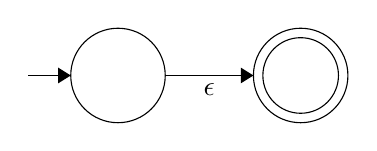
\begin{tikzpicture}[scale=0.2]
\tikzstyle{every node}+=[inner sep=0pt]
\draw [black] (23.5,-19) circle (3);
\draw [black] (35.1,-19) circle (3);
\draw [black] (35.1,-19) circle (2.4);
\draw [black] (26.5,-19) -- (32.1,-19);
\fill [black] (32.1,-19) -- (31.3,-18.5) -- (31.3,-19.5);
\draw (29.3,-19.5) node [below] {$\epsilon$};
\draw [black] (17.8,-19) -- (20.5,-19);
\fill [black] (20.5,-19) -- (19.7,-18.5) -- (19.7,-19.5);
\end{tikzpicture}\\
	a 				& \\
	$R_1 | R_2$ 	& \\
	$R_1 \cdot R_2$ & \\
	$R^*$ 			& \\
	$(R)$ 			& \\
\end{tabular}

\section{Week of August 28th, 2016}
\section{Week of September 4th, 2016}
\section{Week of September 11th, 2016}
\section{Week of September 18th, 2016}
\section{Week of September 25th, 2016}
\section{Week of October 2nd, 2016}
\section{Week of October 9th, 2016}
\section{Week of October 16th, 2016}
\section{Week of October 23rd, 2016}
\section{Week of October 30th, 2016}
\section{Week of November 6th, 2016}
\section{Week of November 13th, 2016}
\section{Week of November 20th, 2016}
\section{Week of November 27th, 2016}

\end{document}